\documentclass[letterpaper,11pt,twocolumn]{article}
\title{Development of traces generator for ARM processor}
\author{Jeoffrey Spinoza, Kunal Patel and Surenkumar Nihalani}
\usepackage{graphicx}



\begin{document}
\maketitle
\section{Abstract}
Memory hierarchy is an important factor in systems design. In order to inform decisions as to what hardware improvements can be made to to a computer architecture, it is necessary to simulate execution of practical programs on that architecture and obtain timing data. There is no way to define the memory hierarchy and simulate the structure of CPU and measure the time. We do have simulators that allow us to define the model, take the program as input and calculate the execution time of the program. For such simulators, you need assembly instruction and the simulator doesn't execute the code, it just simulates the access and write times. Hence, it is a code inspection software. We need to run the program and get all the instructions executed. once, we have the instructions, we can use the timing simulator to find out the metrics of performance of the cpu. The purpose of our software is to extract the list of executed instructions with register accesses and memory access from the emulator for input into timing simulators. Our focus is to develop such a tool for an ARM emulator.
\section{Introduction}
The purpose of this project is to make use of the prexisting CPU simulator, QEMU, to create software that will facilitate execution of test programs on instances of the ARM and x86 architectures, in order to generate traces for input into a timing simulator for architectural study. This project is being carried out by Kunal Patel, Jeoffrey Spinoza, and Surenkumar Nihalani under guidance of Dr. Hyesoon Kim, and with assistance from Mr. Chad Kersey.
\section{Qsim}
\subsection{Usage}
The project is being carried out with the assistance of Mr. Chad Kersey, creator of QSim. QSim is an API, built upon QEMU, designed for helping computer architecture researchers create simulation applications. QSim already provides substantial functionality for running simulations of the x86 architecture. The work at the beginning of the semester was focused on creating a program that would make use of the QSim API to generate traces of program execution on the x86 architecture. Since all of the needed simulation infrastructure was already provided by the QSim API, the focus was on formatting of the traces and gaining familiarity with QSim from a user point of view.
The basic functionalities provided by the QSim library include the ability to instantiate a virtual machine, which, for the interests of this project, consists of the memory and registers visible to the ISA of that virtual machine. Upon instantiation, the virtual machine’s RAM is initialized with a kernel image provided by the user of QSim. QSim also allows any test programs to be loaded into the simulated RAM, providing compilation of the program into the ISA of the virtual machine.
\begin{figure*}
\begin{center}
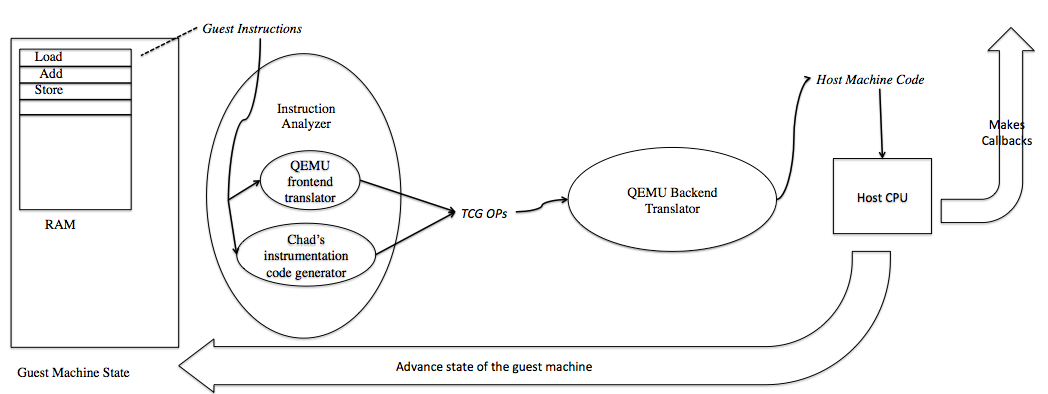
\includegraphics[width=6.5in]{Slide}
\caption{Guest Machine modification process}
\label{fig:f1}
\end{center}
\end{figure*}

After the virtual machine is instantiated, useful operations can be performed on 
this machine. The machine can be told to execute a specific number of 
instructions in its memory. Also particular registers and memory locations can 
be read and written to, independent of instruction execution.
The most powerful feature of the QSim virtual machine instantiation functionality, which is also of key interest to this project, is callback support. While execution of a guest program (a program that resides in the memory of the virtual machine) advances, for every guest instruction executed, the simulation backend takes note of key events that occur in the virtual architecture. These events include the instruction execution itself, register access, interrupts, memory access, and I/O. QSim allows its users to associate callback functions with these these events. The user writes the callback functions, and pointers to these functions are then specified as parameters for the instantiation of the simulated machine. The simulation backend ensures that whenever one of the aforementioned events occurs, a callback to the appropriate user-specified function will be made, allowing information about the guest instruction that was just executed to be passed back up to the user as parameters to these callbacks. Callback support in QSim provides users with a means of gathering large amounts of simulation data with minimal effort, therefore, applications developed for this research project are implemented primarily through the callback mechanism.

\subsection{Dynamic Recompiler}
This section of the document is is concerned with how program execution on the guest machine is implemented. Some understanding of this process is helpful for extending QSim for ARM simulations. Most of the implementation is realized in the QEMU source. When the virtual machine is instantiated it is known as the guest machine, while the computer on which QSim is being run, is called the host machine. The virtual machine’s RAM is known as guest RAM, and instructions that reside in guest RAM are called guest instructions. As stated in section “Chad made QSim, and it is so cool”, one of the methods of the guest machine, is the ability to advance execution of guest instructions, causing realistic changes to take place in the guest memory and registers.
To implement these changes to the guest machine state, the backend uses a method called binary translation. Essentially, the guest instructions are analyzed dynamically, as the guest program advances, and “converted” into the machine code of the host machine (the machine on which QSim is running). In the context of the current project, that means the guest machine has an ARM assembly code program residing in its memory, and during execution, the dynamic re-compiler is converting these instructions into x86 machine code, putting the machine code into a translation cache to be executed directly on the hardware of the host machine. The conversion process involves generating x86 instructions that will change the actual host memory locations in which the guest memory and registers reside,  effectively advancing the state of the of the guest machine according to the semantics of the guest instructions.
\begin{figure*}
\begin{center}
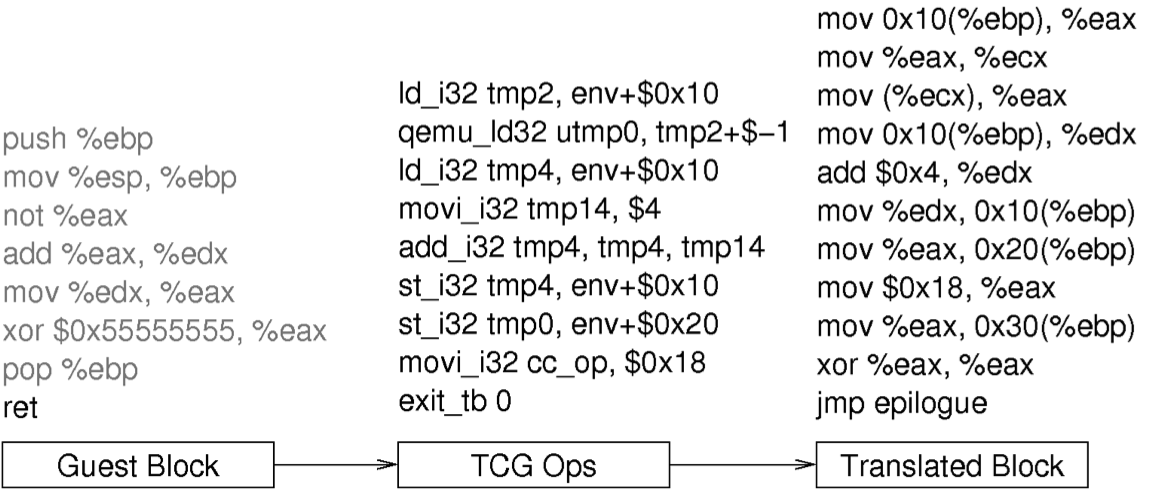
\includegraphics[width=6.5in]{return}
\caption{Guest code to TCG-ops to host code translation}
\label{fig:f2}
\end{center}
\end{figure*}

The entire dynamic recompilation process occurs in two phases. As shown in figure <x>, the instructions are first translated, by the instruction analyzer, into an intermediate representation, called TCG-OPs. TCG ops are the intermediate instructions understood by QEMU's Tiny Code Generator, then from the TCG-OPs, the host code is generated.
To support the callback functionality described in section “Chad made QSim and it is so cool”, the dynamic translation algorithm must be modified so that in addition to generating TCG-OPs that express the semantics of the guest instructions, it will also insert TCG-OP instrumentation code into the translation stream to make callbacks. See section “Callback Implementation” for a more detailed description of the necessary modifications and what has already been done.
\section{x86 Trace Generator Client Program}
Chad wrote the client program known as utrace.cpp (Refer to Appendix A) that helped us understand the working QSim and the problem statement of this project. The file uses the API callbacks of QSim and writes the traces in a file.
\section{QSIM for ARM}
\subsection{Overview and Completed Work}
The focus of the latter portion of the semester, and the focus of future work on this project is on developing a version of QSim software that supports instantiation of a simulated ARM machine.  This requires some modifications to a branch of the QSim source code and installation scripts, and modifications to the board file of the QEMU source, most of which is already completed. The following is a list of those completed tasks:
\begin{itemize}
  \item{Set up Linux cross-compile environment for compiling programs in ARM.}
  \item{Modify board file (<qemu directory>/hw/integrator.c)}
  \item{Code an ARM kernal loader}
  \item{modify getqemu.sh, located in the QSim root directory, to build ARM QEMU}
\end{itemize}
In addition to the steps listed above, considerable modification must be made to the source code of QEMU to create an ARM version of QEMU to serve as the CPU emulator of this ARM version of QSim. QEMU is designed to support simulation of a range of architectures, including ARM, and x86. However, in the creation of QSim, modifications to the QEMU source were made by Chad Kersey to implement the memory access, register access, and callback functionalities discussed the section “Usage”. These modifications were made with consideration to the x86 architecture. To implement support for ARM, similar modifications must be made with consideration of the ARM architecture.  The modifications to QEMU can be organized into the following high-level tasks (relevant files and directories in parenthesis):
\begin{itemize}
	\item{Write memory and register access instructions $(''<qemu directory>/target-arm/op\_helper.c'')$}
	\item{$Add support for the following callbacks:
	(Three files in ''<qemu directory>/target-arm/'' directory: ''op\_helper.c'', ''translate.c'', ''helpers.h'')$
		\begin{itemize}
		\item{Instructions executed}
		\item{Register Access}
		\item{Interrupt}
		\item{Memory Access}
		\item{Atomic instructions executed}
		\item{Magic instruction}
		\end{itemize}
	}
\end{itemize}
Work on the first task has begun. The relevant code modifications can be scene in appendix ''x''. The second task is detailed in the following section.
\subsection{Callback implementation}
One important functionality to be implemented for ARM QSim is callbacks. There are six callbacks to be implemented for ARM and they are listed in the previous section. Implementing callbacks involves work in three files located in
<qemu directory>/target-arm The files are translate.c, op\_helper.c, helpers.h. Translate.c embodies a portion of QEMU’s ''dynamic recompiler'', which we explain in section ''Dynamic Recompiler''. In the translate.c file, there is code that calls functions to generate the appropriate TCG-OPs for each instruction. As stated before, the creators of QSim already implemented translation of ARM instructions into TCG-OPs. However, callbacks have not been implemented, so the code needs to be modified so that the appropriate callbacks will be inserted into the TCG-OP stream as well. In addition, helper functions must be added to the file op\_helper.c, which will actually perform the callbacks by calling the  function pointers set by the user. During translation of guest instructions, TCG-OPs must be generated whose semantics are a function call that references one of the helper functions written in op\_helper.c (whichever one cooresponds to the desired callback). Consult documentation on QEMU to see what the format of the TCG-OPs are.
The magic instruction callback provides a means for guest operating system to perform out of bounds communication. The magic instruction callback gets executed whenever a “magic instruction” is executed in the guest machine code. For x86 simulation, the magic instruction is a CPUID instruction which serves no practicle purpose, so it can be inserted in the guest code for the purpose of callback generation. A similar useless instruction must be selected as the magic instruction for the ARM architecture and the appropriate code in translate.c must be modified to handle translating this instruction into a magic callback.
\end{document}
